\documentclass[man,floatsintext,draftall]{apa6}
\usepackage{lmodern}
\usepackage{amssymb,amsmath}
\usepackage{ifxetex,ifluatex}
\usepackage{fixltx2e} % provides \textsubscript
\ifnum 0\ifxetex 1\fi\ifluatex 1\fi=0 % if pdftex
  \usepackage[T1]{fontenc}
  \usepackage[utf8]{inputenc}
\else % if luatex or xelatex
  \ifxetex
    \usepackage{mathspec}
  \else
    \usepackage{fontspec}
  \fi
  \defaultfontfeatures{Ligatures=TeX,Scale=MatchLowercase}
\fi
% use upquote if available, for straight quotes in verbatim environments
\IfFileExists{upquote.sty}{\usepackage{upquote}}{}
% use microtype if available
\IfFileExists{microtype.sty}{%
\usepackage{microtype}
\UseMicrotypeSet[protrusion]{basicmath} % disable protrusion for tt fonts
}{}
\usepackage{hyperref}
\hypersetup{unicode=true,
            pdftitle={The production of negation in parents' and children's speech},
            pdfauthor={Masoud Jasbi, Annika Mcdermott-Hinman, Kathryn Davidson, \& Susan Carey},
            pdfkeywords={negation, production, child language},
            pdfborder={0 0 0},
            breaklinks=true}
\urlstyle{same}  % don't use monospace font for urls
\usepackage{graphicx,grffile}
\makeatletter
\def\maxwidth{\ifdim\Gin@nat@width>\linewidth\linewidth\else\Gin@nat@width\fi}
\def\maxheight{\ifdim\Gin@nat@height>\textheight\textheight\else\Gin@nat@height\fi}
\makeatother
% Scale images if necessary, so that they will not overflow the page
% margins by default, and it is still possible to overwrite the defaults
% using explicit options in \includegraphics[width, height, ...]{}
\setkeys{Gin}{width=\maxwidth,height=\maxheight,keepaspectratio}
\IfFileExists{parskip.sty}{%
\usepackage{parskip}
}{% else
\setlength{\parindent}{0pt}
\setlength{\parskip}{6pt plus 2pt minus 1pt}
}
\setlength{\emergencystretch}{3em}  % prevent overfull lines
\providecommand{\tightlist}{%
  \setlength{\itemsep}{0pt}\setlength{\parskip}{0pt}}
\setcounter{secnumdepth}{0}
% Redefines (sub)paragraphs to behave more like sections
\ifx\paragraph\undefined\else
\let\oldparagraph\paragraph
\renewcommand{\paragraph}[1]{\oldparagraph{#1}\mbox{}}
\fi
\ifx\subparagraph\undefined\else
\let\oldsubparagraph\subparagraph
\renewcommand{\subparagraph}[1]{\oldsubparagraph{#1}\mbox{}}
\fi

%%% Use protect on footnotes to avoid problems with footnotes in titles
\let\rmarkdownfootnote\footnote%
\def\footnote{\protect\rmarkdownfootnote}


  \title{The production of negation in parents' and children's speech}
    \author{Masoud Jasbi\textsuperscript{1}, Annika Mcdermott-Hinman\textsuperscript{2}, Kathryn Davidson\textsuperscript{2}, \& Susan Carey\textsuperscript{2}}
    \date{}
  
\shorttitle{Child and Parent Production of Negation}
\affiliation{
\vspace{0.5cm}
\textsuperscript{1} UC Davis\\\textsuperscript{2} Harvard University}
\keywords{negation, production, child language\newline\indent Word count: X}
\usepackage{csquotes}
\usepackage{upgreek}
\captionsetup{font=singlespacing,justification=justified}

\usepackage{longtable}
\usepackage{lscape}
\usepackage{multirow}
\usepackage{tabularx}
\usepackage[flushleft]{threeparttable}
\usepackage{threeparttablex}

\newenvironment{lltable}{\begin{landscape}\begin{center}\begin{ThreePartTable}}{\end{ThreePartTable}\end{center}\end{landscape}}

\makeatletter
\newcommand\LastLTentrywidth{1em}
\newlength\longtablewidth
\setlength{\longtablewidth}{1in}
\newcommand{\getlongtablewidth}{\begingroup \ifcsname LT@\roman{LT@tables}\endcsname \global\longtablewidth=0pt \renewcommand{\LT@entry}[2]{\global\advance\longtablewidth by ##2\relax\gdef\LastLTentrywidth{##2}}\@nameuse{LT@\roman{LT@tables}} \fi \endgroup}


\usepackage{lineno}

\linenumbers

\authornote{Add complete departmental affiliations for each author here. Each new line herein must be indented, like this line.

Enter author note here.

Correspondence concerning this article should be addressed to Masoud Jasbi, 469 Kerr Hall, University of California, One Shields Avenue, Davis, CA, 95616. E-mail: \href{mailto:jasbi@ucdavis.edu}{\nolinkurl{jasbi@ucdavis.edu}}}

\abstract{
this is the abstract


}

\begin{document}
\maketitle

\hypertarget{introduction}{%
\section{Introduction}\label{introduction}}

Under Construction!

\hypertarget{previous-studies}{%
\subsection{Previous Studies}\label{previous-studies}}

Klima and Bellugi (1966) provided the first and most influential account of negation development. They used fortnightly recordings of mother-child conversations for three children in the Brown (1973) corpus: Eve (18-26 months), Adam and Sarah (26-50 months). They divided child utterances into three stages:\enquote{the first stage from the first month of study for each child; the last from the month in which the MLUs approach 4.0 for each of the three children; and the second stage between the two.} They suggested that in Stage 1, the syntactic category of negation (NEG) includes \emph{no} and \emph{not}, produced before or after a sentence \enquote{nucleus}, i.e.~noun and verb phrase without tense or inflection (NEG+S or S+NEG). Examples include: \enquote{No singing song}, \enquote{No the sun shining}, \enquote{No money}, \enquote{No play that}, \enquote{Wear mitten no}, \enquote{No fall!}, and \enquote{Not a teddy bear}. It was hypothesized that auxiliary negatives like \emph{don't} and \emph{can't} are not produced or understood at this stage. In Stage 2, children add \emph{can't} and \emph{don't} as unanalyzed wholes to their list of negators, and move negation inside the sentence, between the subject and the verb phrase (NP+NEG+VP). The main evidence for \emph{can't} and \emph{don't} being unanalyzed wholes in this stage is the absence of positive auxiliary variants like \emph{can} and \emph{do}. Typical examples at this stage include \enquote{I can't see you}, \enquote{I don't want it}, \enquote{He not little, he big}, \enquote{There no squirrels}, \enquote{He no bite you}, and \enquote{I no want envelope}. In Stage 3, auxiliary verbs like \emph{can't} and \emph{don't} are re-analyzed as AUX+NEG, additional negative auxiliaries like \emph{won't} and \emph{isn't} are produced, and positive auxiliaries like \emph{can} and \emph{do} are produced for the first time (NP+AUX+NEG+VP). Klima and Bellugi (1966)'s account was in line with the transformational theory of negation at the time, which hypothesized that adult negation starts as a sentence modifier at deep structure, and a transformation later moves it inside the sentence (Klima, 1964). Therefore, children's first stage was interpreted to reflect a universal innate initial state, and the second and third stages the process of learning the required surface-level transformations.

However, further investigations proved the first stage to be controversial. Bloom (1970) studied another three children (Kathryn, Eric, and Gia) between 19-27 months and did not find evidence for a sentence-external stage of negation (NEG+S / NEG+S). Children started with isolated \emph{no} and once they produced multi-word utterances, they mostly combined \emph{no} and \emph{not} with noun and verb phrases (\emph{no}/\emph{not}+NP/VP). Nevertheless, Bloom (1970) reported that Kathryn produced some instances of sentence-internal negation with \emph{no} such as \enquote{Kathryn no like celery}. Lord (1974) studied her own child Jennifer (19-26 months) and found no instances of sentence-external negation or sentence-internal \emph{no}. She reported that her child started with single \enquote{no} utterances before 24 months and between 24-26 months started combining \emph{no}/\emph{not} with nominals, and \emph{can't}/\emph{don't} with verb phrases (\emph{no}/\emph{not}+NP and \emph{can't}/\emph{don't}+VP). Her conclusion was that the development of negation varies in children and not all of them go through the stages described by Klima and Bellugi (1966).

However, Wode (1977) used crosslinguistic data to support and expand Klima and Bellugi (1966)'s account. He compared productions of two German children (19-26 months), a Swedish child (20-42 months) from Lange and Larsson (1973), and English-speaking children from Bloom (1970) and Klima and Bellugi (1966). He proposed four stages: 1. one-word stage with only \emph{nein}, \emph{nä/nej}, or \emph{no}; 2. multiword anaphoric stage where the single words from stage 1 are used as a response to a previous utterance followed by other words (e.g. \enquote{no, outside!} or \enquote{nein, Milch}); 3. multiword non-anaphoric stage where a single-word negative like \emph{no} is used sentence-externally instead of sentence-internally (e.g. \enquote{nein sauber} for \enquote{I don't want to be cleaned} or \enquote{no close} for \enquote{I can't close the box}) 4. multiword intra-sentential negation where negation has moved inside the sentence (e.g. \enquote{Kathryn no like celery}, \enquote{I can't open it}, or \enquote{ich habe nicht geschlafen}). In response to this proposal, Park (1979) argued that Wode (1977)'s account relied on insufficient evidence given that it used only 13 examples and no proper distributional analysis. Furthermore, Park (1979) presented data from three German speaking children around 21-25 months that did not match Wode (1977)'s developmental stages.

The debate continued with de Villiers and de Villiers (1979) suggesting that previous studies provided little empirical evidence to support a general sentence-external stage. They investigated productions of Adam (27-31 months), Eve (18-22 months), and their own child Nicholas (23-29 months) and found very few sentence-external negatives with overt subjects that allowed for assessment of sentence boundary. They pointed out that even among these instances, many could plausibly be anaphoric. Despite these arguments, Déprez and Pierce (1993) used examples from children's productions in English, French, and German to provide a novel syntactic analysis for presenential negation in child language within the Principles and Parameters framework (Chomsky, 1993). They argued that instead of negation moving from outside the sentence inside as Klima and Bellugi (1966) suggested, it is the subject NP that fails to move outside, from inside the VP. They suggested that child data is in line with the VP-internal subject hypothesis in adult grammar (Koopman \& Sportiche, 1991). However unlike previous studies, they had counted utterances with omitted subjects as instances of presentential negation (or rather VP-internal subjects) as well.

In response to Déprez and Pierce (1993), Stromswold and Zimmermann (2000) studied negation in five German-speaking children (Julia, Inga, Andreas, Kathrin, and Nicole) between 17 and 29 months. They found that out of 689 examples of negation, only one could plausibly support the hypothesis that at an early stage the negator can surface to the left of the subject and pre-sententially. Drozd (1995) provided a similar but large-scale analysis for English. Using data available from 123 children in CHILDES between the ages of 11 and 40 months, the study looked at utterances beginning with \emph{no}, \emph{not}, and \emph{never} and used the available linguistic context to classify them as anaphoric or non-anaphoric. The study found a total of 456 instances of pre-sentential negation, out of which only 31 (6.7\%) could be classified as instances of non-anaphoric pre-sentential negation. He argued that the best explanation for such rare distribution of presentential negation is that they are meta-linguistic uses of negation. In other words, the child's \enquote{no the sun shining} is similar to the adult version \enquote{don't say the sun is shining (that's wrong)}, and not some stage in the development of negation.

Two relatively recent studies have focused on Klima and Bellugi (1966)'s second stage, where children are reported to produce non-adult-like infinitival negatives with \emph{no}, \emph{not}, and \emph{don't} (e.g. \enquote{He no/not/don't bite you}). At this stage, children are hypothesized to not differentiate these forms and consider all as variants of negation. They are also hypothesized to not analyse \emph{don't} as auxiliary plus negation and rather consider it as an unanalyzed whole. The evidence was considered to be the absence of positive auxiliary forms like \emph{do}. Schütze (2010) provided a quantitative analysis of negation in the speech of five children (Abe, Adam, Sarah, Nina, Ross) between 2 and 5 years of age. He showed that the non-adult-like infinitival negatives are quite rare, never exceeding 5\% of children's total productions. Instead he found that the only common error reaching about 10\% of productions is non-agreeing \emph{don't} in sentences with third-person singular subjects (e.g. \enquote{He don't bite you}). He proposed a grammatical account that could predict such errors.

Thornton and Tesan (2013) disagreed with Schütze (2010) and following Klima and Bellugi (1966) contended that children at the second stage have not yet identified \emph{n't} as a separate form of negation. To explain this stage, they proposed that children start with the hypothesis that negative words like \emph{not}, \emph{not}, and \emph{don't} are adverbs, thus producing sentences like \enquote{He no/not/don't bite you}. Later in the third stage they realize that negation can also be a separate syntactic head showing agreement with subjects as in \enquote{He doesn't bite you}. This analysis was inspired by Zeijlstra2004's proposal for Negative Concord which divides languages into those with adverbial semantic negation and those with syntactic negation. Thornton and Tesan (2013) provided elicitation data on negative sentences with third-person singular subjects from four two-year-olds who had been recorded for about a year (Tesan, 2005). They found that in line with their proposal, children produced \emph{not} (e.g. \enquote{This not fits in here}) before producing \emph{n't} (e.g. \enquote{this does not fit in here}). A similar finding regarding the order in which negative morphmes emerge in English was reported by Cameron-Faulkner, Lieven, and Theakston (2007). They investigated the development of multiword negation in the speech of Brian (2;3-3;4, MLU 2.05-3.1) and reported that negative morphemes followed a \emph{no}\textless{}\emph{not}\textless{}\emph{n't} trajectory, mirroring their order of frequency in parents' speech. Earliest multiword negation strategies were \enquote{\emph{no}/\emph{not}+XP} utterances, with \emph{don't} and \emph{can't} being the first contracted forms to emerge.

To summarize, prevoius research has suggested that English-speaking children learn to produce negative morphemes in a \emph{no}\textless{}\emph{not}\textless{}\emph{n't} order. Among negative auxiliary forms, \emph{can't} and \emph{don't} are learned first and before any positive auxiliary form including \emph{can} and \emph{do}. Klima and Bellugi (1966) argued that children's production of English negation becomes adult-like after two non-adult-like stages: one in which they produce negation before a sentence and never inside it, and another in which they produce it within the sentence but do not use the right negative morpheme (e.g. \enquote{He not little} instead of \enquote{He isn't little}). There has been an active debate over each of these stages. With the exception of Drozd (1995), previous studies have mainly relied on data from a few available children often including the original data from Klima and Bellugi (1966). Given that over the years much more corpus data and computational tools have become available, it is important to revisit previous proposals and assess their current status.

\hypertarget{current-study}{%
\subsection{Current Study}\label{current-study}}

This paper builds on the rich literature on children's production of negation by bringing the largest dataset of English parent-child interactions available in CHILDES (MacWhinney, 2000). Study 1 investigates the frequency of production for each negative morpheme in parents' and children's speech during the first 6 years of children's development. More specifically the study checks to see if there is an overall \emph{no} \textless{} \emph{not} \textless{} \emph{n't} cline (Cameron-Faulkner et al., 2007), and if children produce negative auxiliary forms like \emph{can't} and \emph{don't} before their positive variants like \emph{do} and \emph{can}. Study 2 focuses on non-adult-like productions of negation in children and examines the prevalence of pre-sentential negation (e.g. \enquote{no the sun shining}) as well as infinitival negation (e.g. \enquote{He no/not/don't bite you}). It also discusses the concept of stagehood and whether observed prevalances of such non-adult-like productions are best captured as a developmental stage. Study 3 looks for the most common negative syntactic structures present in parents' and children's speech. It uses a current state-of-the-art parsing algorithm to provide a large-scale estimate of syntactic structures negation participates in as well as its productivity in parent-child interactions. We end with a discussion of English negation's combinatorial capacity in children's early speech and its possible origins.

\hypertarget{study-1-development-of-negative-morphemes}{%
\section{Study 1: Development of Negative Morphemes}\label{study-1-development-of-negative-morphemes}}

The aim of this study was to assess the overall production of negative forms (especially \emph{no}, \emph{not}, and \emph{n't}) in parents' and children's speech, and address the following questions: 1. Does the overall production of negation in children follow a \emph{no}\textless{}\emph{not}\textless{}\emph{n't} cline (Cameron-Faulkner et al., 2007)? 2. Do children produce negative auxiliary forms such as \emph{can't} and \emph{don't} before using their positive variants, suggesting that the negative forms are learned as unanalyzed wholes? The answer to both questions was negative.

\hypertarget{methods}{%
\subsection{Methods}\label{methods}}

For samples of parents' and children's speech, we used the online database \href{childes-db.stanford.edu}{childes-db} and its associated R programming package \texttt{childesr} (Sanchez et al., 2019). Childes-db is an online interface to the child language components of \href{https://talkbank.org/}{TalkBank}, namely \href{https://childes.talkbank.org/}{CHILDES} (MacWhinney, 2000) and \href{https://phonbank.talkbank.org/}{PhonBank}. Two collections of corpora were selected: English-North America and English-UK. The dataset contained 14,195,967 tokens from 571 children, after necessary exclusions. We ran a token-based analysis of the corpora as well as an utterance-based analysis that could take utterance length and context into account.

In our token-based analysis, all word tokens were tagged for the following information: 1. the speaker role (parent vs.~child), 2. the age of the child when the word was produced in months, 3. whether the word was positive or negative, and 4. the type of negative word produced. For this study we considerd the following classes of negative morphemes in English: the forms \emph{no} and \emph{not}, all instances of negative auxiliary forms with \emph{n't} as well as their positive forms without \emph{n't} as controls. Unintelligible tokens were excluded (N = 402,117), as well as tokens that had missing information on children's age (N = 1,057,287). Third, tokens outside the age range of 1 to 6 years were excluded (N = 542,304) since children did not produce much outside this age range. These exclusions resulted in the exclusion of data 100 children from the final analysis. Similarly, in our utterance-based analysis, each utterance was tagged for the following: 1. the number of tokens in the utterance 2. the speaker role (parent vs.~child), 2. the age of the child, 3. whether the utterance contained \emph{no}, \emph{not}, or \emph{n't}. Utterances with missing information on children's age (N = 379,399) as well as those outside the age range of 1 to 6 years were excluded (N = NULL). The collection contained X utterances from N children.

\hypertarget{results}{%
\subsection{Results}\label{results}}

We first look at the proportions of different categories of negation in parents' and children's speech (Figure \ref{fig:negationProportionPlot}). The most frequent form in parents' speech was the contracted auxiliary negation \emph{n't}, followed by \emph{no}, and finally \emph{not}. In children's productions and between the ages of 12-18 months, almost all negative forms are instances of \emph{no}, with some contracted auxiliary negatives like \emph{don't} and \emph{can't}. As children grow older, the proportions of \emph{not} and its contracted form \emph{n't} increase while the proportion of \emph{no} decreases. Similar to Cameron-Faulkner et al. (2007) we find that children start productions of \emph{no} earlier than other forms. However, we do not find evidence that the full form \emph{not} is produced before its contracted form \emph{n't}. The results in Figure \ref{fig:negationProportionPlot} suggest that children start producing \emph{not} and \emph{n't} around the same time, if not slightly earlier for \emph{n't}.

\begin{figure}
\centering
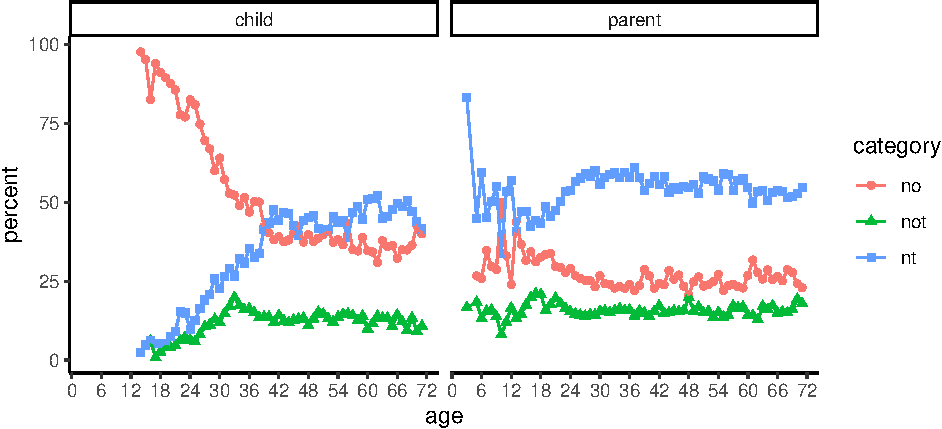
\includegraphics{negation_production_files/figure-latex/negationProportionPlot-1.pdf}
\caption{\label{fig:negationProportionPlot}Proportion of different categories of negation in parents' and children's speech between 1 to 6 years of age.}
\end{figure}

Figure \ref{fig:negationRelativeFrequency} shows the relative frequency of the morphemes \emph{no}, \emph{not} and \emph{n't} per thousand words in the speech of parents and children. Children start producing \emph{no} between 12-18 months and they immediately surpass their parents' rate of production for this morpheme. Betwen 18-42 months children produce two to three times more instances of \emph{no} than their parents. This rapid incrase and high frequency of \emph{no} may be partly because parents ask many yes/no questions from children in this age range. After 42 months the frequency of \emph{no} reduces substantially and gets closer to parents' level of 10 per thousand. For the negative morpheme \emph{not}, children start their productions between 12-24 months and by 30 months of age, they are producing \emph{not} at the same rate as their parents (5 per thousand words). After 36 months children's rate of \emph{not} productions stay similar to their parents. Finally for the contracted form \emph{n't}, children's productions start between 12-18 months and by 24 months they reach a rate of 5 instances per thousand words. They keep increasing this rate until they reach their parents' rate of 15 instances per thousand at age 36 months. It is important to note that for all these negative forms, children have reached a substantial level of production by 30 months of age.

\begin{figure}
\centering
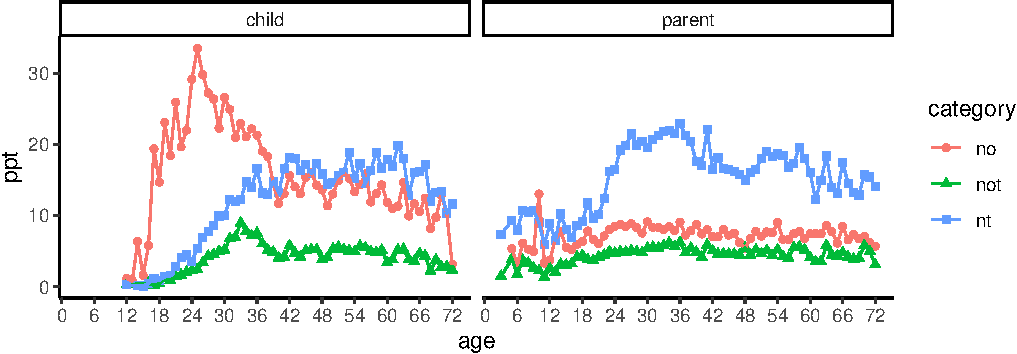
\includegraphics{negation_production_files/figure-latex/negationRelativeFrequency-1.pdf}
\caption{\label{fig:negationRelativeFrequency}Relative frequency (parts per thousand) of the response particle \emph{no}, verb phrase negation \emph{not}, and its contracted form \emph{n't}}
\end{figure}

Stromswold and Zimmermann (2000) found that in German-speaking children, the word \emph{nein} was produced before \emph{nicht} and discussed three potential causes for this order of production: input frequency, phonetic complexity, and syntactic complexity. They explained that input frequency cannot be the cause because in German-speaking children's input \emph{nicht} was more frequent than \emph{nein}. Similarly, English-speaking children hear more instances of \emph{n't} than \emph{no} so input frequency cannot be the cause in English either. With respect to phonetic complexity, German \emph{nicht} has a voiceless palatal fricative that can potentially be hard for children and delay its production. However, English \emph{no} and \emph{not} are quite similar and do not contain phones that are known to be particularly hard for children. This leaves us with syntactic complexity which is an obvious difference between isolated one-word negators like \emph{no}/\emph{nein} and multiword negators like \emph{not}/\emph{nicht}. Given that children start with shorter utterances (typically one word) and produce longer ones as they grow up, they may produce \emph{no} earlier than \emph{not} and \emph{n't} simply because \emph{no} can appear as a single word utterance. In other words, even a hypothetical child that comprehends all negative forms \emph{no}, \emph{not}, and \emph{nt} may produce \emph{no} earlier than the other two because of production limitations.

One way to address this issue in our dataset is to focus on children's multiword utterances. Is the main contributor to the high frequency of \emph{no} single word utterances? To answer this question we removed single-token utterances like \enquote{yes}, \enquote{no}, and \enquote{oh}, as well as utterances that combined such elements in a repetitive way like \enquote{no no} or \enquote{oh no} from children and parents' speech. If early appearance and high frequency of \emph{no} is mainly due to short and repetitive utterances produced by children early in their development, it should disappear once we focus on multiword utterances. As Figure \ref{fig:multiwordFrequency} shows, this is largely what we found. While the frequencies of \emph{not} and \emph{n't} in multi-word productions were similar to their overall frequencies seen before in Figure \ref{fig:negationRelativeFrequency}, the word \emph{no} largely lost its advantage in frequency and early occurrence, showing a very similar developmental trajectory as the other two negative morphemes. This provides an indication that the earlier emergence of \emph{no} may be due to children's production limitations and does not necessarily reflect earlier acquisition of this morpheme. The question of which form is acquired earlier may be better addressed by careful comprehension studies in the 12-24 month age range. It is important to note here that both Figure \ref{fig:multiwordFrequency} and Figure \ref{fig:negationRelativeFrequency} suggest that the 12-18 months age range is a crucial period where all three negative morphemes recieve their early form-meaning mappings.

\begin{figure}
\centering
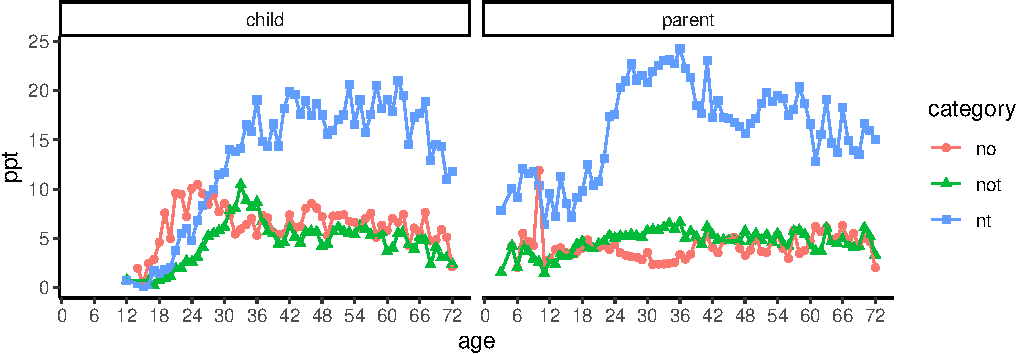
\includegraphics{negation_production_files/figure-latex/multiwordFrequency-1.pdf}
\caption{\label{fig:multiwordFrequency}Relative frequency (parts per thousand) of the response particle \emph{no}, verb phrase negation \emph{not}, and its contracted form \emph{n't} in multiword utterances}
\end{figure}

Moving to the second question: do negative auxiliaries appear before positive ones? Figure \ref{fig:auxRelFreq} shows the relative frequency of positive and negative auxiliary forms in the speech of children and their parents. Our results show that overall, children start producing the positive and negative auxiliary forms around the same time and always produce the positive forms at a higher rate than negative ones. This is also true for individual auxiliary words such as \emph{do/don't} and \emph{can/can't} which are produced earlier than others. Therefore, the claim that negative auxiliary forms are produced before their positive counterparts is not supported by the available production data and consequently production data does not support the hypothesis that auxiliary negative forms are learned as unanalyzed wholes.

\begin{figure}
\centering
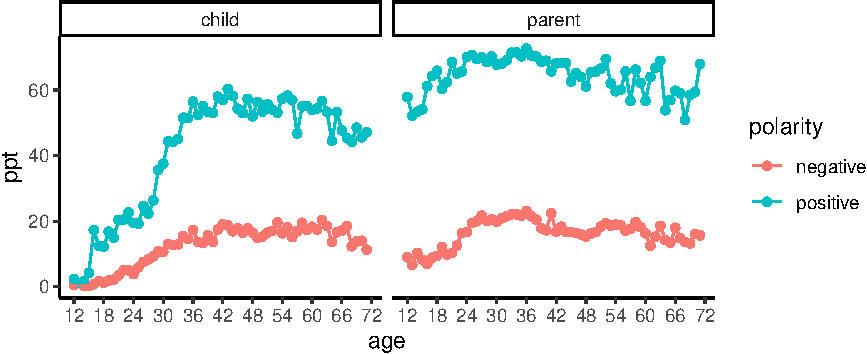
\includegraphics{negation_production_files/figure-latex/auxRelFreq-1.pdf}
\caption{\label{fig:auxRelFreq}Relative frequency (parts per thousand) of positive auxiliary forms such as \emph{do}, \emph{are}, and \emph{can} as well as their contracted negatives in the speech of parents and children.}
\end{figure}

\hypertarget{conclusions}{%
\subsection{Conclusions}\label{conclusions}}

The results of our corpus study suggest that children produce \emph{no} earlier and more frequently than \emph{not} and \emph{n't}. We did not find strong evidence for \emph{not} appearing before \emph{n't} and the general trends suggested that they appear around the same time. While earlier emergence of \emph{no} in production may suggest its earlier acquisition and comprehension, it is also possible that early emergence of \emph{no} is due to its syntactic and usage properties. The morpheme \emph{no} can be produced on its own as a speech act in response to speech participants, while negative forms \emph{not} and \emph{n't} require composition with other words. We found that when we consider only children's multiword utterances, the early emergence and advantage of \emph{no} disappears. Therefore, the production data does not provide support for some strong order or stage of acquisition in children's acquisition of negative morphemes. We believe it is more appropriate for future comprehension research to adjudicate this matter.

We also investigated whether negative auxiliary forms such as \emph{can't} and \emph{don't} emerge before their positive counterparts such as \emph{do} and \emph{can}. Previous research had cited such a phenomenon as evidence for the proposal that negative auxiliary forms are first learned as unanalyzed wholes. Contrary to previous reports, our data showed that the positive auxiliary forms emerge around the same time as the negative ones but produced much more frequently. Therefore, production data does not provide evidence for negative auxiliaries being learned as unanalyzed forms.

\hypertarget{study-2-non-adult-like-productions}{%
\section{Study 2: Non-adult-like Productions}\label{study-2-non-adult-like-productions}}

The aim of this study was to assess the prevalence of non-adult-like utterances in children's productions. Klima and Bellugi (1966)'s account of negation development relies on two types of non-adult-like utterances: 1. Pre-sentential instances where a negative morpheme is modifying a sentence (NEG + NP + VP); and 2. Intra-sentential instances where in some cases fails to show the adult-like agreement (NP + \emph{no}/\emph{not}/\emph{don't} + VP). How prevalent are such errors and what are their most likely sources?

\hypertarget{method}{%
\subsection{Method}\label{method}}

\hypertarget{results-1}{%
\subsection{Results}\label{results-1}}

\hypertarget{conclusion}{%
\subsection{Conclusion}\label{conclusion}}

\hypertarget{study-3-early-syntactic-structures-for-negation}{%
\section{Study 3: Early Syntactic Structures for Negation}\label{study-3-early-syntactic-structures-for-negation}}

In this study we ask what syntactic analyses can be attributed to children's early negative utterances. We also ask what common syntactic structures are present in parents' speech. The goal is to provide an account of children's syntactic development in the spirit of Klima and Bellugi (1966)'s pioneering work with data and computational tools available today.

\hypertarget{method-1}{%
\subsection{Method}\label{method-1}}

\hypertarget{results-2}{%
\subsection{Results}\label{results-2}}

\hypertarget{general-discussion}{%
\section{General Discussion}\label{general-discussion}}

So far: Our results are compatible with emergence of negation around 18-24 months, converging with studies on comprehension of negation.

\newpage

\hypertarget{acknowledgments}{%
\section{Acknowledgments}\label{acknowledgments}}

\hypertarget{declaration-of-interest-statement}{%
\section{Declaration of Interest Statement}\label{declaration-of-interest-statement}}

\hypertarget{references}{%
\section{References}\label{references}}

\hypertarget{appendices}{%
\section{Appendices}\label{appendices}}

The auxiliary category in our previous figures lump together a wide variety of auxiliary verbs that develop at different rates. Figure \ref{fig:AuxWords} shows the production of common negative auxiliary verbs in the speech of children and parents, sorted from top-left to bottom-right based on frequency. The most frequent negative auxiliary form in child-directed speech is \emph{don't} and it is also the earliest and most frequent auxiliary form in children's speech. Children start producing it between 12-24 months and they quickly reach the parents' rate at 36 months. Perhaps the fastest development occurs with the auxiliary \emph{can't}. Children start producing it between 18-24 months and very quickly surpass their parents' rate.

\begin{figure}
\centering
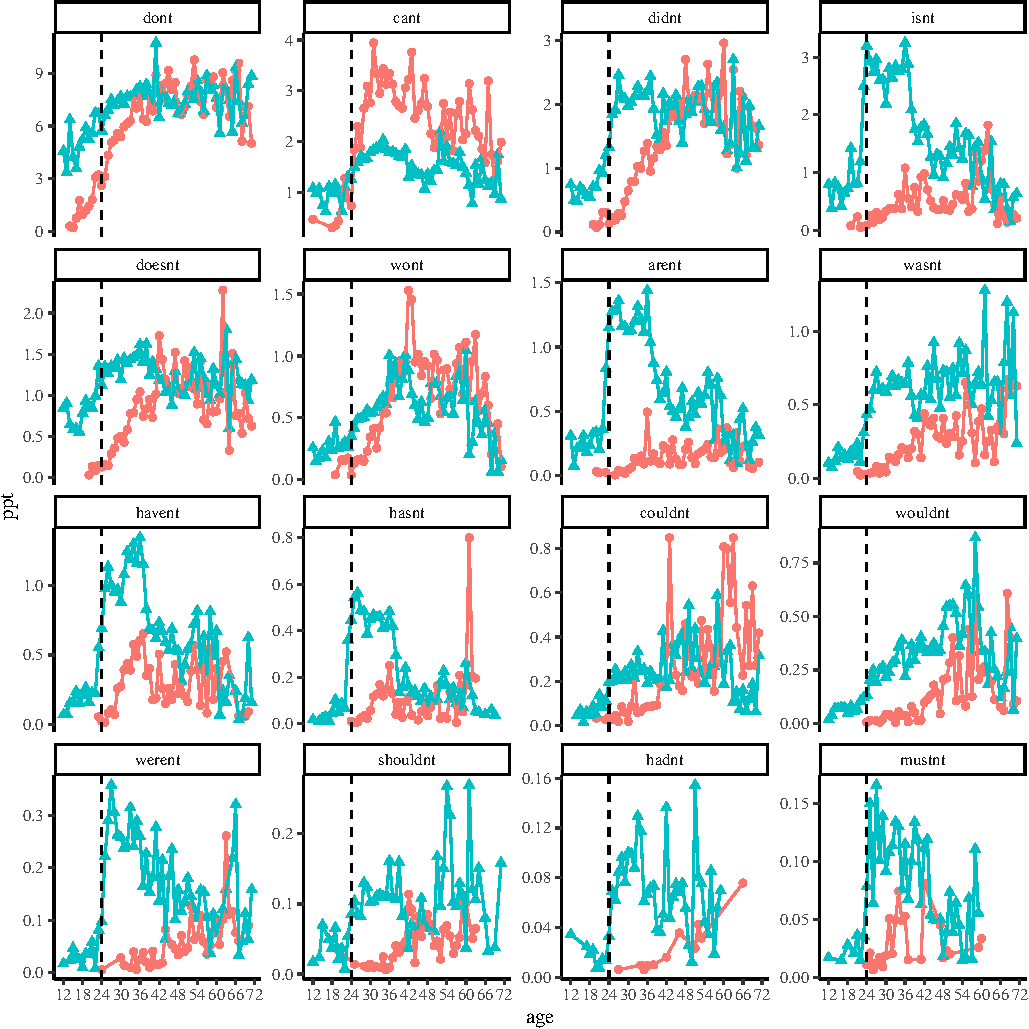
\includegraphics{negation_production_files/figure-latex/AuxWords-1.pdf}
\caption{\label{fig:AuxWords}Relative frequency of negated auxiliary verbs in the speech of parents (green triangles) and children (red circles). The dashed line marks 24 months on the x axis.}
\end{figure}

Figure \ref{fig:pronouns} shows the development of negative and positive indefinite pronouns: \emph{everything}, \emph{nothing}, \emph{something}. Children start producing these words quite early as well, with \emph{nothing} reaching the parent level of production at 30 months.

\begin{figure}
\centering
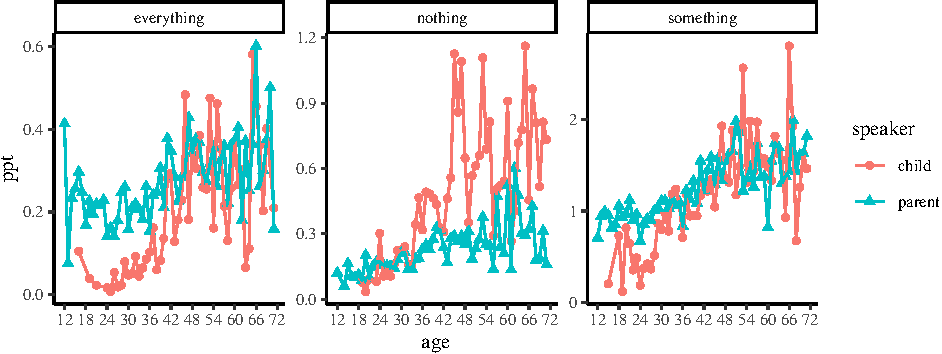
\includegraphics{negation_production_files/figure-latex/pronouns-1.pdf}
\caption{\label{fig:pronouns}Relative frequency of pronouns \emph{everything}, \emph{something}, and \emph{nothing}}
\end{figure}

\begin{figure}
\centering
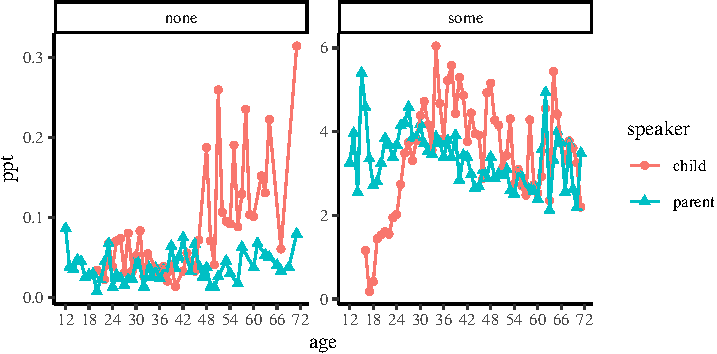
\includegraphics{negation_production_files/figure-latex/quantifiers-1.pdf}
\caption{\label{fig:quantifiers}Relative frequency of quantifeirs \emph{none}, \emph{some}, and \emph{all}.}
\end{figure}

Adverbs of frequency

\begin{figure}
\centering
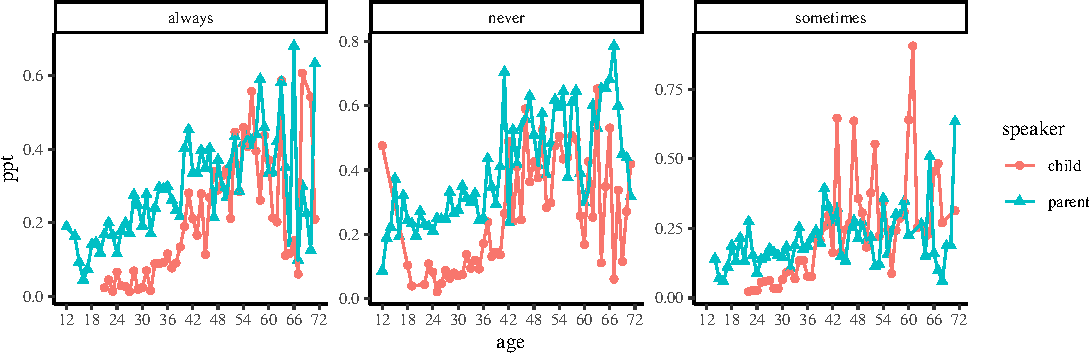
\includegraphics{negation_production_files/figure-latex/adverbs-1.pdf}
\caption{\label{fig:adverbs}Relative frequency for adverbs of frequency \emph{always}, \emph{never}, and \emph{sometimes} in the speech of parents and children.}
\end{figure}

\begingroup
\setlength{\parindent}{-0.5in}
\setlength{\leftskip}{0.5in}

\endgroup

\hypertarget{refs}{}
\leavevmode\hypertarget{ref-bloom1970}{}%
Bloom, L. M. (1970). \emph{Language development: Form and function in emerging grammars.} Cambridge, MA: MIT press.

\leavevmode\hypertarget{ref-brown1973first}{}%
Brown, R. (1973). \emph{A first language: The early stages.} Harvard U. Press.

\leavevmode\hypertarget{ref-cameron2007part}{}%
Cameron-Faulkner, T., Lieven, E., \& Theakston, A. (2007). What part of no do children not understand? A usage-based account of multiword negation. \emph{Journal of Child Language}, \emph{34}(2), 251.

\leavevmode\hypertarget{ref-chomsky1993lectures}{}%
Chomsky, N. (1993). \emph{Lectures on government and binding: The pisa lectures}. Walter de Gruyter.

\leavevmode\hypertarget{ref-deVilliers1979}{}%
de Villiers, P. A., \& de Villiers, J. G. (1979). Form and function in the development of sentence negation. \emph{Papers and Reports on Child Language Development}, \emph{17}, 57--64.

\leavevmode\hypertarget{ref-deprez1993negation}{}%
Déprez, V., \& Pierce, A. (1993). Negation and functional projections in early grammar. \emph{Linguistic Inquiry}, 25--67.

\leavevmode\hypertarget{ref-drozd1995}{}%
Drozd, K. F. (1995). Child english pre-sentential negation as metalinguistic exclamatory sentence negation. \emph{Journal of Child Language}, \emph{22}(3), 583--610.

\leavevmode\hypertarget{ref-klima1964negation}{}%
Klima, E. (1964). Negation in english. The structure of language, ed. By ja fodor and jj katz, 246-323. Englewood Cliffs, NJ: Prentice-Hall.

\leavevmode\hypertarget{ref-klimaBellugi1966}{}%
Klima, E. S., \& Bellugi, U. (1966). Syntactic regularities in the speech of children. In \emph{Psycholinguistics papers} (pp. 183--207). Edinburgh University Press.

\leavevmode\hypertarget{ref-koopman1991position}{}%
Koopman, H., \& Sportiche, D. (1991). The position of subjects. \emph{Lingua}, \emph{85}(2-3), 211--258.

\leavevmode\hypertarget{ref-lange1973syntactical}{}%
Lange, S., \& Larsson, K. (1973). Syntactical development of a swedish girl, embla, between 20 and 42 months of age, part i: Age 20-25 months. \emph{Project Child Language Syntax}.

\leavevmode\hypertarget{ref-lord1974variations}{}%
Lord, C. (1974). Variations in the acquisition of negation. \emph{Papers and Reports on Child Language Development}, \emph{8}, 78--86.

\leavevmode\hypertarget{ref-macwhinney2000childes}{}%
MacWhinney, B. (2000). \emph{The CHILDES project: The database} (Vol. 2). Mahwah, NJ: Erlbaum.

\leavevmode\hypertarget{ref-park1979some}{}%
Park, T.-Z. (1979). Some facts on negation: Wode's four-stage developmental theory of negation revisited. \emph{Journal of Child Language}, \emph{6}(1), 147--151.

\leavevmode\hypertarget{ref-sanchez2019childes}{}%
Sanchez, A., Meylan, S. C., Braginsky, M., MacDonald, K. E., Yurovsky, D., \& Frank, M. C. (2019). Childes-db: A flexible and reproducible interface to the child language data exchange system. \emph{Behavior Research Methods}, \emph{51}(4), 1928--1941.

\leavevmode\hypertarget{ref-schutze2010status}{}%
Schütze, C. T. (2010). The status of nonagreeing don't and theories of root infinitives. \emph{Language Acquisition}, \emph{17}(4), 235--271.

\leavevmode\hypertarget{ref-StromswoldZimmermann2000}{}%
Stromswold, K., \& Zimmermann, K. (2000). Acquisition of nein and nicht and the vp-internal subject stage in german. \emph{Language Acquisition}, \emph{8}(2), 101--127.

\leavevmode\hypertarget{ref-tesan2005children}{}%
Tesan, G. M. (2005). \emph{What do children have in their heads? Functional heads and parameter setting in child language} (PhD thesis).

\leavevmode\hypertarget{ref-thorntonTesan2013}{}%
Thornton, R., \& Tesan, G. (2013). Sentential negation in early child english. \emph{Journal of Linguistics}, 367--411.

\leavevmode\hypertarget{ref-wode1977four}{}%
Wode, H. (1977). Four early stages in the development of li negation. \emph{Journal of Child Language}, \emph{4}(1), 87--102.


\end{document}
